

\section{Justification of feature scoping}

\subsection{One feature in-scope:}
The command-line interface feature is considered as in-scope for our system as it is the most fundamental way for an operator to be able to interact with the system. Since the rest of the system (Control station and robot) do not themselves give any value to a customer because of their nature in acting upon assigned missions and other commands given from an operator source. Without such instructions there would be no robot activity, there would also be no way for the customers to know anything regarding the robot positions nor have any knowledge regarding the arbitrary reward point score.

\subsection{One feature out-of-scope:}
Viewing the camera feed from the robot in a graphical interface would be a feature which is not within the scope of our intended product yet something that could be incorporated if the need for it would arise. The robots do possess the ability to capture a feed through the use of their camera component, and in the simulator we see the camera feed being displayed. What this feature would bring is that camera feed provided to the operator for what could be exploratory purposes, as well as a tool used in an  eventual manual control feature.



\section{Description of implemented features in more detail}

The features currently implemented within the system are as follows:
\begin{itemize}
    \item Command line: The command line interface for the operator to use when they wish to assign missions or send instructions to the robots. Although not all such functionality is yet implemented it has placeholder functions already in place to be filled out when it is time for the specific feature to be implemented.\newline The command line interface shows the current reward points as well as a few options for different inputs, such as the assigning of missions and instructions which are relayed to the robot, as well as an input for updating the interface so as to fetch new data from the control station storage.
    A future addition to this style of interface could be the introduction of a map showing the positions of robots within certain areas using ASCII symbols. The ASCII symbols would 'draw' a map and update the robot positioning when the update function is called.
    \item Graphical interface: Another alternative to the command line interface is the graphical interface which has similar functionality in a more stylised and user friendly format so that a customer might sell it to a wider audience. It has buttons for the different actions which can be taken, these actions are the same ones which are present in the command line interface, with the possibility of adding dynamic updating so as to more smoothly relay information updates from the robots to the operator.
    \item Emergency stop: Both interfaces can use the implemented emergency stop function which we classify as an 'Instruction'. This Instruction is relayed from the operator interface and relayed to the control station which then sends it forth to the robot. The robot in turn handles this Instruction by accessing the appropriate routine for emergency stopping and as such enters a state where it stays in position without being able to move as it is fed the same coordinate in the effort to give the robot no room to execute a move another move command.
    \item Change colour: This feature allows the operator to change a robot's colour at any time. This can be done through both the command-line and the graphical user interfaces. This feature can be used as a way to mark specific robots which might be intended for different purposes such as executing missions with a unique strategy. As such the changing of colour can be used to differentiate robot purposes and group together robots for such purposes.
    
\end{itemize}


\section{Changes to existing diagrams}
\begin{enumerate}
    \item action.do renamed to action.execute due to do being a reserved word in java
    \item Place routines in their own subbackage to increase readability
    \item Method renames of Actuator and Sensor interfaces due to name clashed with the simulator
    \item Add constructors for easier initialisation of the control station
    \item Display holds a refference to the opertaor interface
    \item Made the model imutable, thus removing and and adding some methods.
    \item Put interfaces to interfaces
    \item Better names for point rewarder subsystem
    \item Add a graphical user interface
    \item Remove most classes in the console user interface, just leaving one class to handle the IO loop
\end{enumerate}

\section{Contribution}

\begin{itemize}
    \item Philip Nord 
       \begin{itemize}
           \item Finalising the skeleton code in order to get the Emergency Instruction to work so the chain between a call from user-interface and all the way to the simulator is done.
           \item Implemented the control stations storage functionality.
       \end{itemize}
    \item William Lev\'{e}n
       \begin{itemize}
           \item Implemented the change colour feature
           \item Finalising the skeleton code in order to get the Emergency Instruction to work so the chain between a call from user-interface and all the way to the simulator is done.
           \item Refurbished the console application for demo usage.
       \end{itemize}
    \item Svante Bennhage
       \begin{itemize}
           \item Deciding on a structure on a feature model diagram as well as implementation of it.
           \item Further implementation and structure of the Point Rewarder class.
       \end{itemize}
    \item Sebastian Fransson
       \begin{itemize}
           \item Deciding on a structure on a feature model diagram as well as implementation of it.
           \item Writing the main parts of the report.
       \end{itemize}
    \item Victor Johansson
       \begin{itemize}
           \item Analysed the feature model to notice if something were missing.
           \item Finalising the skeleton code in order to get the Emergency Instruction to work so the chain between a call from user-interface and all the way to the simulator is done.
       \end{itemize}
    \item Snezhina Racheva
       \begin{itemize}
           \item Deciding on a structure on a feature model diagram as well as implementation of it.
           \item Implemented a GUI for demo purposes.
       \end{itemize}
\end{itemize}

\begin{figure}
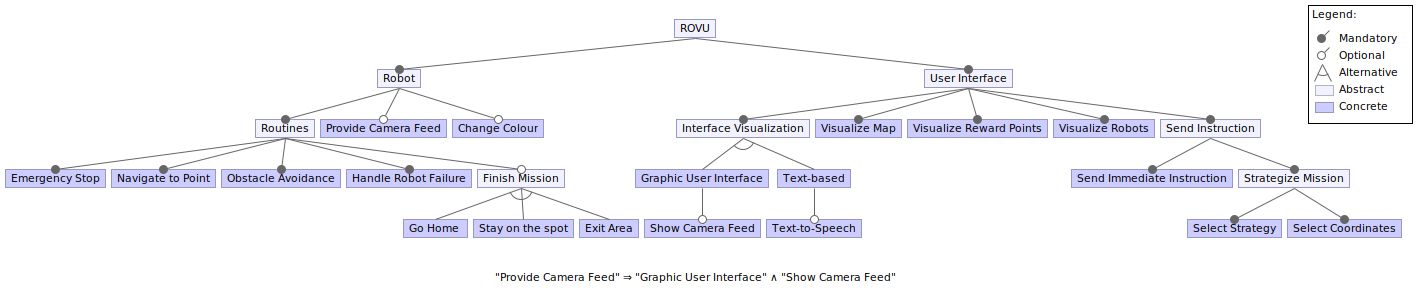
\includegraphics[width=22cm, angle=-90]{docs/assignments/Assignment_4/diagram.png}
\end{figure}